\documentclass[12pt,letterpaper,english]{article}
\usepackage[round, authoryear]{natbib}
\usepackage{floatrow}
\renewcommand{\floatpagefraction}{.99}
\newfloatcommand{capbtabbox}{table}[][\FBwidth]
\usepackage{eurosym}
\usepackage{graphicx}
\usepackage{setspace}
\usepackage{geometry}
\usepackage{bbm}
\usepackage{hyperref}
\usepackage[titletoc]{appendix}
\usepackage{graphicx}
\newcommand{\argmin}{\arg\!\min}
\usepackage{amsmath, amssymb,amsthm,mathtools,dsfont}
\usepackage{algorithmic}
\usepackage{booktabs}
\usepackage{setspace}
\usepackage{enumerate}
\usepackage[flushleft]{threeparttable}
\usepackage{rotating}
\usepackage{float}
\usepackage{tabulary}
\usepackage{ragged2e}
\usepackage{rotating}
\usepackage{epstopdf}
\usepackage[labelfont=bf]{caption}
\usepackage{array}
\newcolumntype{C}[1]{>{\centering\let\newline\\\arraybackslash\hspace{0pt}}m{#1}}
\usepackage{subfig}
\usepackage{placeins}
\usepackage{pxfonts}
\usepackage{xcolor}
\usepackage{svg}
\usepackage{multirow}
\usepackage{verbatim}
\usepackage{soul}
\sethlcolor{yellow}
\hypersetup{
	colorlinks,
	linkcolor={red!50!black},
	citecolor={red!50!black},
	urlcolor={blue!80!black}
}
\textheight=23cm \textwidth=16.5cm \oddsidemargin=0cm
\evensidemargin=0cm \topmargin=-1.75cm
\setcounter{MaxMatrixCols}{10}
\makeatletter
\g@addto@macro\@floatboxreset\centering
\makeatother
\setlength\floatsep{2\baselineskip plus 3pt minus 2pt}
\setlength\textfloatsep{2\baselineskip plus 3pt minus 2pt}
\setlength\intextsep{2\baselineskip plus 3pt minus 2 pt}
\newcommand*{\MyIndent}{\hspace*{0.5cm}}%
\usepackage[normalem]{ulem}
\newtheorem{theorem}{Proposition}
\newtheorem{definition}{Definition}
\newtheorem{proposition}{Proposition}
\newtheorem{corollary}{Corollary}
\newtheorem{example}{Example}
\newtheorem{lemma}{Lemma}
\newtheorem{remark}{Remark}
\newtheorem{assumption}{Assumptions}
\newtheorem{hypothesis}{Hypothesis}


% Uncomment the next line to use the harvard package with bibtex
%\usepackage[abbr]{harvard}

% This command determines the leading (vertical space between lines) in draft mode
% with 1.5 corresponding to "double" spacing.
%\draftSpacing{1.5}
%\newlength\TableWidth
\usepackage{array}
\newcolumntype{H}{>{\setbox0=\hbox\bgroup}c<{\egroup}@{}}
\newcommand{\Figures}{Figures/}
\newcommand{\Tables}{Tables/}
\usepackage{pifont}
\newcommand{\cmark}{\ding{51}}%
\newcommand{\xmark}{\ding{55}}%

\title{\textbf{Response to Referee 1\\ Quantitative Economics MS 2442 \\``Welfare and Spending Effects of \\ Consumption Stimulus Policies''}}
\author{Christopher D. Carroll, Edmund Crawley, William Du, \\ Ivan Frankovic, and H\aa kon Tretvoll}
\date{}

\begin{document}
	\onehalfspacing
	\maketitle
	
\noindent Thank you for your thoughtful comments and suggestions on our paper ``Welfare and Spending Effects of Consumption Stimulus Policies''. They were all very useful to us in revising the paper. We hope you agree that the paper has improved. In the following, we summarize the main changes we have made based on your, the other referees', and the editor's suggestions. Thereafter, we state each of your comments in italics and provide point-by-point responses to them.

\section{Summary of Main Changes}

\begin{itemize}
	\item \textbf{The Splurge}
	\item \textbf{Welfare Measure} We have completely overhauled our section on welfare and have introduced a new measure that we think best captures the idea that we want to measure welfare gains from carrying out each policy during a recession, but give no benefit in normal times to policies that in our model would increase welfare through redistribution. 
	
	Our welfare measure weights the felicity of a household at time $t$ by the marginal utility of the same household in a counterfactual simulation in which neither the recession occurred nor the fiscal policy was implemented. This weighting scheme means that in normal times the marginal benefit to a social planner of moving a dollar of consumption from one household at one time period to another household at the same or different time period is zero. Hence, in normal times, any re-distributive policy has zero marginal benefit. However, in a recession when the average marginal utility is higher than in normal times, there can be welfare benefits to government borrowing to allow households to consume more during the recession.
	
	Our new welfare measure leads to the same qualitative conclusions as in the previous version of the paper. It improves on the previous measure in several ways:
	\begin{itemize}
		\item The new measure does not scale with the size of the fiscal stimulus. We divide by the net present value of the fiscal policy so the measure is a `bang-bang-for-the-buck' measure. As pointed out by referee 2, our previous measure was biased by the change in the size of the UI extension policy in a recession relative to normal times.
		\item Our new measure more naturally removes the bias to policies that redistribute from high to low-marginal utility households in normal times. Previously, we took away the welfare benefit in normal times of each policy. In our new measure, ANY marginal redistributive policy has no welfare benefit in normal times.
		\item One benefit of removing the splurge from our household behavior is that our welfare measure now matches with the utility function in the households' optimization problem.
	\end{itemize}
	For more details on how we treat welfare, see section \colorbox{yellow}{XX}.
	
	\item \textbf{Robustness in a General Equilibrium Model}  The main results of this paper are presented in a partial equilibrium setup with aggregate demand effects that do not arise from a general equilibrium setup. We think there are many advantages to studying the welfare and multiplier effects in this setting without embedding the model in general equilibrium.
	
	However,  we now complement our analysis with a  general equilibrium HANK model, as standard as possible, but able to capture supply-side effects that are absent from the partial equilibrium setup and to introduce a fiscal rule to balance the government budget. We find that the consumption multipliers across horizons follow the same qualitative pattern as we have in our partial equilibrium analysis.
	
	The write up of this HANK model is found in section \colorbox{yellow}{XX}
	
	
\end{itemize}

\newpage 

\section{Essential points}
\begin{enumerate}
	\item \textit{\textbf{Partial equilibrium.} The main drawback of the analysis is the partial equilibrium nature. \citet{kekre2022unemp} and Broer et al (2023), in contrast, seem to find general-equilibrium effects to be important. I think the PE approach still gives interesting results, but the authors should be more up-front about it (the word "partial equilibrium" appears first on page 11), and discuss its shortcomings.}
	
	\noindent \textbf{Response.} As described above in the "Summary of Main Changes," we now include a section that analyzes the behavior of our households when embedded in a simple HANK and SAM model. We have also changed the introduction to make clear our approach and both some advantages and disadvantages of working with a partial equilibrium model.
	
	\item \textit{\textbf{Tax policy.} Do taxes rise eventually to pay for the policies? I don't think so, but this is extremely unclear. ``Should'' appears four times in the discussion of the financing of government policies. The authors should introduce an explicit rule for tax policy (even if paid very far in the future), as this may matter for consumption of the Ricardian / high-wealth households.}
	
	\noindent \textbf{Response.} In our primary partial equilibrium analysis, we do not model the fiscal rule. This is now clear in the text, ``To keep our analysis as simple as possible, we do not model the debt repayment.''  The main insight that has come from the new generation of HA models is that business-cycle-frequency dynamics are little affected by alternative choices about debt repayment; we could have modeled a half-life of the fiscal target of 15 years or 50 years without changing the results meaningfully, so introducing a discussion of the various choices about the fiscal rule and making a case for one or another choice did not seem to us a good use of the reader's time. However, in our general equilibrium HANK model we do include a fiscal rule ensuring that the level of government debt returns to its steady-state level slowly over time.
	% [x] CDC elaborated
	
	\item \textit{\textbf{`Splurge' and utility.} The implications of splurge consumption should be discussed more in detail. Take, e.g., the assumption that households gain utility only from post-splurge consumption. This implies that, essentially, the model is equivalent to an alternative where all incomes are taxed by 30 percent (and immediately go into government consumption). But doesn't this increase further, and mechanically, the effect of transfers to the low-wealth unemployed (who consume post-splurge income, increasing marginal utility by 1/0.7=1.42 relative to that from total income) relative to high-wealth households (who consume permanent income from financial wealth)?}
		
	\noindent \textbf{Response.} As described above in the "Summary of Main Changes," we now include a section that discusses the relevance of the splurge for our results. We show that with a wider distribution of discount factors even a model without the splurge is able to account for the relevant empirical evidence. Our main results, including the ranking of the polices in terms of welfare impact, are robust to removing the splurge from the model. 

	\item \textit{\textbf{Calibration of the `splurge'.} I find the calibration strategy, to estimate the `splurge' on Norwegian data (plus a US liquid-wealth distribution...), and then calibrate the rest to US data only, confusing - also since the authors then compare their final average annual MPC to an estimate for Norway. I would appreciate a clear motivation for why we need the Norwegian data targets at the beginning of Section 3.1 - I guess it's because we don't have estimates for MPCs by wealth for the US. An alternative, perhaps cleaner, calibration would be to US data only with some sensitivity analysis for alternative values of the splurge-fraction. In any case, I would appreciate a (perhaps only verbal) comparison to the more common `share-of-hand-to-mouth-agents' calibration (that doesn't capture wealthy high-MPC agents but may have similar demand properties).}
	
	\noindent \textbf{Response.} Our model captures the high proportion of hand-to-mouth agents by matching the liquid wealth distribution comprehensively and not only at a specially designated (and somewhat arbitrary). The attempt in earlier models to measure a share of hand-to-mouth consumers was a start to the more comprehensive exercise of matching the entire distribution of liquid wealth.
	
	As described above in the "Summary of Main Changes," our main conclusions also hold in an estimated model of the US economy where the splurge is set to zero. These results are derived entirely without use of Norwegian data, as that data is only used in the estimation of the splurge. As such, the calibration strategy using both US and Norwegian data has no bearing on our ultimate results. Nevertheless, we now more clearly and prominently spell out at the beginning of section 3 that the use of Norwegian data, as your rightly guess, results from a lack of comparable empirical evidence for the US (or anywhere else, so far as we know). 
	
\bigskip
\bigskip

\item \textit{\textbf{Additional comments}} 

	\begin{enumerate}
		\item \textit{\textbf{Clarification of the calibration.} I didn't understand if the model is for households, or individuals, and what data target pertains to which of the two (the text uses both words, although "household" dominates).}
		
		\noindent \textbf{Response.} Our model is a simplified model of households. This fits with our calibration to the distributions of liquid wealth from the SCF which is a survey of families in the US. It is simplified, however, in that we do not take into account heterogeneity across household size or composition. The classification of households into three education groups is based on the level of education of the head of the household. The income risk and employment/unemployment transitions can also be thought of as applying to the head of the household as the calibration targets from the Bureau of Labor statistics are for unemployment rates and duration for individuals. However, we take into account that the model is for a household in the calibration of the replacement rates with or without unemployment benefits. The parameters describing the unemployment system is based on \citet{rothstein2017scraping} who study the effects of unemployment on household income. 
		
		In response to your comment, we have clarified our presentation of the calibration. 
		
		\item \textit{\textbf{Additional policies.} To give the payroll tax cut a better chance, couldn't the authors consider a ``payroll tax cut as long as the recession lasts''? And I don't understand why the authors don't consider an increase in UI generosity, which also is a common policy.}
						
		\noindent \textbf{Response.} We do not consider a payroll tax cut that only applies during a recession as we view it as unlikely that policy makers would implement such a policy. The end date of a recession is only identified with a significant lag by the NBER Business Cycle Dating Committee. A tax cut that was a function of this retrospective dating of a recession by the committee would then imply a tax increase (reversal of the tax cut) with potentially several months of retroactive effect. In the model, the tax cut could, of course, expire as soon as the economy transitioned out of the recession, but this option does not seem available in practice. 
		
		One reason we have focused on the policy of extending instead of expanding UI benefits is that the policies we consider are motivated by policies implemented in the aftermath of the Great Recession, and the Tax Relief, Unemployment Insurance Reauthorization, and Job Creation Act of 2010 included an extension of federal unemployment benefits. Although an increase in UI generosity is also a policy that has been applied, for example the CARES act implemented during the COVID-19 pandemic included both extension and expansion of benefits, we view the extension of eligibility for benefits as the more common policy. 
		
		It is also worth noting the point made by \citet{ganongConsumer2019} that UI extensions is likely to be the more important policy. The considerable drop in spending upon the expiry of unemployment benefits that they identify leads them to conclude that ``the consumption-smoothing gains from extending UI benefits are four times greater than from increasing the level of UI benefits'' (page 2384).
		
		Our framework could be extended to also consider a policy of making UI benefits more generous. At the moment, our code is not set up to do that, however, and while changing the codes to include this policy would be relatively straightforward, it would be computationally costly to recompute all our results for an additional policy. 

		Finally, in the robustness section included in this version, where we consider some of the general equilibrium effects of stimulus policies in a HANK and SAM model, we also considered a policy of increasing UI generosity. We found that the multipliers for a policy of increasing the replacement rates for unemployed households are substantially smaller than those for a policy of extending benefit eligibility. We have not included these results in the paper, but Figure~\ref{fig:multHANKSAM} shows the multipliers from the HANK and SAM model including the policy of increasing UI generosity.
                % not sure that there is a to-do here?
		% [ ] CDC: note that the citation to Ravn and Sterk 2017 is moved to the MainChanges document
		
		\begin{figure}
			\begin{center}
				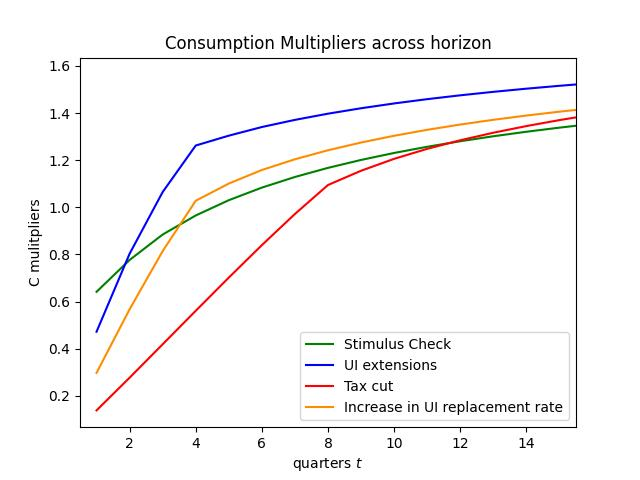
\includegraphics[width=.65\textwidth]{../../../../Code/HA-Models/FromPandemicCode/Figures/HANK_Figures/HANK_multipliers_w_splurge_and_generosity}
				\caption{Multipliers for different policies in the HANK and SAM model}
				\label{fig:multHANKSAM}
			\end{center}			
		\end{figure}
	
		\item \textit{\textbf{Motivation of modeling choices.} Why the two-year horizon for the payroll-tax	reduction? Consumers expect this policy to continue with 50 percent	probability if the recession continues for longer than 2 years. Why?}

		\noindent \textbf{Response.} The two-year horizon for the payroll-tax reduction is inspired by the two-year tax cut implemented in the Tax Relief, Unemployment Insurance Reauthorization, and Job Creation Act of 2010. This tax cut was itself an extension of previously implemented cuts known as the ``Bush tax cuts''. In general, we view it as a significantly easier process for policy makers to extend a tax cut that is in place than to start the legislative process from scratch to implement a new policy. Therefore, we let consumers expect that the policy may continue if the recession outlasts the two-year horizon of the initial tax cut.
		
		In response to your questions, we have added more background for the motivation of our choice of policies in section~2.2 of the paper.  

		\item \textit{\textbf{Consumption drop upon unemployment.} The authors should report the drop in consumption upon unemployment benefit expiry, and compare it to the estimates in \citet{ganongConsumer2019}.}

		\noindent \textbf{Response.} Thank you for this suggestion. We now include a discussion of the consumption drop upon unemployment benefit expiry in our model in section~3.3.3, and we compare this to the result reported in \citet{ganongConsumer2019}. 
	
		\item \textit{\textbf{Why the quarterly calibration?} This implies that the unemployed are at least unemployed for three months, which is high relative to U.S. job-finding rates. The unemployment-rate targets should be adjusted for that.}

		\noindent \textbf{Response.} We chose a quarterly calibration since this is the standard in the literature on business cycles and we explicitly consider policies in response to recessions. We consider it realistic that a recession starts and a policy is implemented within the same period when the period in the model is one quarter.
		
		We don't think the education-specific unemployment rate targets should be adjusted because of the frequency of the model, but we agree that the frequency is important for the interpretation of the probabilities of transitioning into and out of unemployment in our calibration. Further discussion of your comments here is incorporated in the reply to your point below concerning job-finding rates. 
		
		\item \textit{\textbf{Job-finding rates.} Why the homogeneous job-finding rates across education groups and duration? It seems unnecessary (since the model keeps track of individual duration and education) and probably produces counterfactually few low-skill long-term unemployed.}
		
		\noindent \textbf{Response.} Our calibration target for the probability of transitioning from unemployment to employment is the average duration of unemployment. As we are using the 2004 wave of the SCF, we use the average number of weeks unemployed from 2004 from the Bureau of Labor Statistics, which was 19.6 weeks = 4.5 months = 1.5 quarters. With a quarterly model we can match that average, and since we do not have data on education-specific durations of unemployment, we do so by calibrating the transition probability from unemployment to employment to be the same across education groups. With a monthly calibration we would match the same average with a lower transition probability, without the implication that those who become unemployed would remain unemployed for at least three months. 
		
		The education-specific element of our calibration is to target the average unemployment rates by education group. We do so by calibrating education-specific transition probabilities from employment to unemployment. Our calibration strategy is consistent with the results in \citet{mincer1991education} who finds that the main difference between education groups is in the incidence of unemployment, and not its duration. He states that ``the reduction of the incidence of unemployment [at higher education levels] is found to be far more important than the reduced duration of unemployment in creating the educational differentials in unemployment rates'' (page 1). 
		
		\citeauthor{mincer1991education} reports probabilities of transitioning into unemployment as the product of the probability of job separation times the conditional probability of unemployment given a job separation, and both of these are lower for higher education levels. For our calibration, this means that a higher job finding rate \textit{within} the quarter of the job separation for more educated workers translates into a lower probability of transitioning from employment to unemployment during a quarter. In that sense, our calibration is consistent with short-term job-finding rates being higher for more educated workers. 
		
		\citet{mincer1991education} refers to data from 1979 and 1980, and there may have been substantial changes in the labor market since then. However, more recent work by \citet{elsby2010labor} include data up to 2009 and echo \citeauthor{mincer1991education}'s findings (see their Figure 8). 
		
		In response to your questions and comments, we have updated our discussion of the calibration of these transition probabilities in the text and added the references discussed here. 
		
	\end{enumerate}
\end{enumerate}

\bigskip

\noindent Finally, we would like to thank you again for your careful advice on our paper. We hope you find our revision satisfactory.

\bibliographystyle{econark}
\bibliography{../../../../HAFiscal.bib,response}
\end{document}
